\documentclass[12pt,executivepaper]{article}
\usepackage[utf8]{inputenc}
\usepackage[spanish]{babel}
\usepackage{amsmath}
\usepackage{amsfonts}
\usepackage{amssymb}
\usepackage{graphics}
\usepackage{graphicx}
\usepackage[left=1cm,right=1cm,top=2cm,bottom=2cm]{geometry}
\usepackage{imakeidx}
\makeindex[columns=3, title=Alphabetical Index, intoc]
\usepackage{listings}
\usepackage{xcolor}
\usepackage{multicol}
\usepackage{changepage}
\usepackage{float}
\usepackage{cite}
\usepackage{url}
\usepackage{hyperref}
\usepackage{pdfpages}

\definecolor{codegreen}{rgb}{0,0.6,0}
\definecolor{codegray}{rgb}{0.5,0.5,0.5}
\definecolor{codepurple}{rgb}{0.58,0,0.82}
\definecolor{backcolour}{rgb}{0.95,0.95,0.92}

\lstdefinestyle{mystyle}{
    backgroundcolor=\color{backcolour},
    commentstyle=\color{codegreen},
    keywordstyle=\color{magenta},
    numberstyle=\tiny\color{codegray},
    stringstyle=\color{codepurple},
    basicstyle=\ttfamily\footnotesize,
    breakatwhitespace=false,
    breaklines=true,
    captionpos=b,
    keepspaces=true,
    numbers=left,
    numbersep=5pt,
    showspaces=false,
    showstringspaces=false,
    showtabs=false,
    tabsize=3
}

\lstset{style=mystyle}
\author{González Pardo Adrian}
\date{Febrero 2020}

\title{Reporte de practica 3}
\newcommand\tab[1][1cm]{\hspace*{#1}}
\begin{document}
\maketitle
\section{Código VHDL}
\begin{center}
    \lstinputlisting[language=VHDL]{./sources/practica.vhd}
    \textit{Código fuente de sumador con acarreo anticipado}
\end{center}
\section{Test-Bench VHDL Código}
\begin{center}
    \lstinputlisting[language=VHDL]{./sources/simPrac2.vhd}
    \textit{Código de simulación}\\
    \textbf{Anexo de fotos de la simulación a impulsos}
\end{center}

\begin{flushleft}
	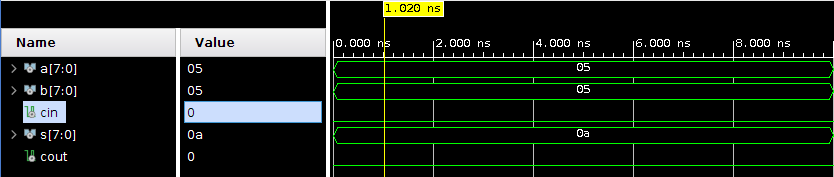
\includegraphics[scale=0.55]{imgs/primera.png}
\end{flushleft}
\begin{center}
    \textit{Primer parte con valores hexadecimales equivales a valores decimales: $a=5{\scriptscriptstyle10}$ $\&$ $b=5{\scriptscriptstyle10}$ con salida $s = A{\scriptscriptstyle16}= 10{\scriptscriptstyle10}$}  
\end{center}

\begin{flushleft}
	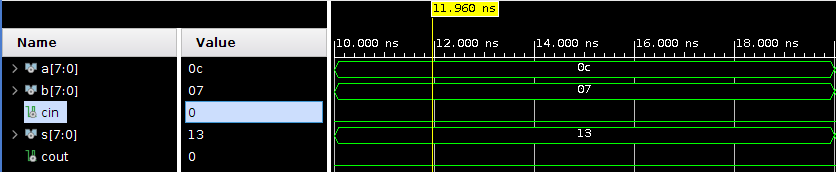
\includegraphics[scale=0.55]{imgs/segunda.png}
\end{flushleft}
\begin{center}
    \textit{Segunda parte con valores hexadecimales equivales a valores decimales: $a=C{\scriptscriptstyle16}=12{\scriptscriptstyle10}$ $\&$ $b=7{\scriptscriptstyle10}$ con salida $s = 13{\scriptscriptstyle16}= 19{\scriptscriptstyle10}$}  
\end{center}

\begin{flushleft}
	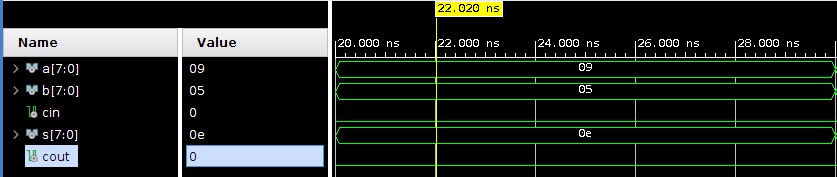
\includegraphics[scale=0.55]{imgs/tercera.png}
\end{flushleft}
\begin{center}
    \textit{Tercer parte con valores hexadecimales equivales a valores decimales: $a=9{\scriptscriptstyle10}$ $\&$ $b=5{\scriptscriptstyle10}$ con salida $s = E{\scriptscriptstyle16}= 14{\scriptscriptstyle10}$}  
\end{center}


\begin{flushleft}
	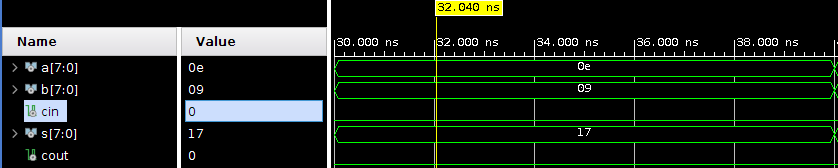
\includegraphics[scale=0.55]{imgs/cuarta.png}
\end{flushleft}
\begin{center}
    \textit{Cuarta parte con valores hexadecimales equivales a valores decimales: $a=E{\scriptscriptstyle16}=14{\scriptscriptstyle10}$ $\&$ $b=9{\scriptscriptstyle10}$ con salida $s =17{\scriptscriptstyle16}=23{\scriptscriptstyle10}$}
\end{center}

\begin{flushleft}
	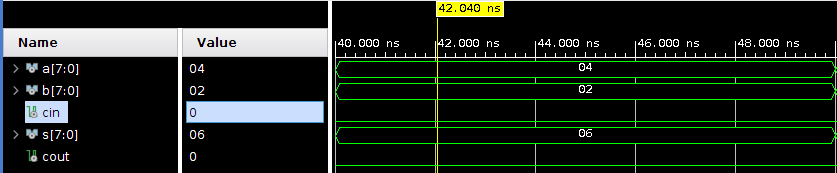
\includegraphics[scale=0.55]{imgs/quinta.png}
\end{flushleft}
\begin{center}
    \textit{Quinta parte con valores hexadecimales equivales a valores decimales: $a=4{\scriptscriptstyle10}$ $\&$ $b=2{\scriptscriptstyle10}$ con salida $s = 6{\scriptscriptstyle10}$}
\end{center}

\begin{flushleft}
	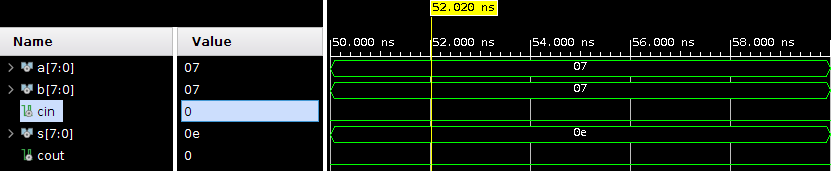
\includegraphics[scale=0.55]{imgs/sexta.png}
\end{flushleft}
\begin{center}
    \textit{Sexta parte con valores hexadecimales equivales a valores decimales: $a=7{\scriptscriptstyle10}$ $\&$ $b=7{\scriptscriptstyle10}$ con salida $s =E{\scriptscriptstyle16}=14{\scriptscriptstyle10}$}
\end{center}

\begin{flushleft}
	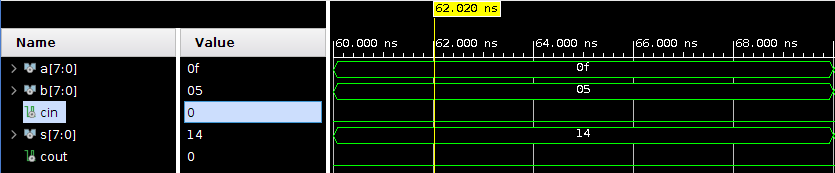
\includegraphics[scale=0.55]{imgs/septima.png}
\end{flushleft}
\begin{center}
    \textit{Septima parte con valores hexadecimales equivales a valores decimales: $a=F{\scriptscriptstyle16}=15{\scriptscriptstyle10}$ $\&$ $b=5{\scriptscriptstyle10}$ con salida $s =14{\scriptscriptstyle16}=20{\scriptscriptstyle10}$}
\end{center}

\begin{flushleft}
	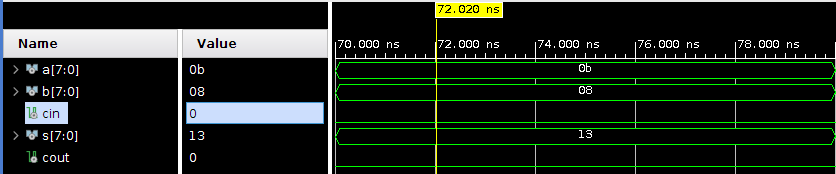
\includegraphics[scale=0.55]{imgs/octava.png}
\end{flushleft}
\begin{center}
    \textit{Octava parte con valores hexadecimales equivales a valores decimales: $a=B{\scriptscriptstyle16}=11{\scriptscriptstyle10}$ $\&$ $b=8{\scriptscriptstyle10}$ con salida $s =13{\scriptscriptstyle16}=19{\scriptscriptstyle10}$}
\end{center}

\begin{flushleft}
	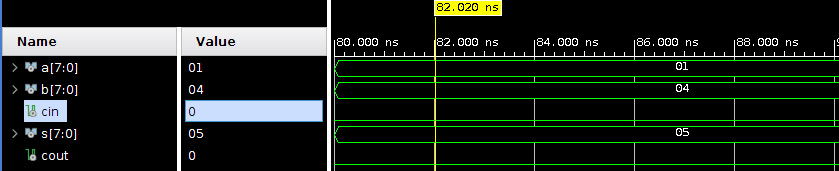
\includegraphics[scale=0.55]{imgs/novena.png}
\end{flushleft}
\begin{center}
    \textit{Novena parte con valores hexadecimales equivales a valores decimales: $a=1{\scriptscriptstyle10}$ $\&$ $b=4{\scriptscriptstyle10}$  con salida $s =5{\scriptscriptstyle10}$}
\end{center}
\section{Tabla de resultados}
\begin{center}
    \begin{tabular}{|p{2cm}|p{2cm}|p{2cm}|p{3cm}|p{2cm}|}
    \hline
    Operación & A & B & S & Cout \\\hline
    Suma & 5 & 5 & 10 & 0\\\hline
    Suma & 12 & 7 & 19 & 0 \\\hline
    Suma & 9 & 5 & 14 & 0 \\\hline
    Suma & 14 & 9 & 23 & 0 \\\hline
    Suma & 4 & 2 & 6 & 0 \\\hline
    Suma & 7 & 7 & 14 & 0 \\\hline
    Suma & 15 & 5 & 20 & 0 \\\hline
    Suma & 11 & 8 & 19 & 0 \\\hline
    Suma & 1 & 4 & 5 & 0 \\\hline
    \end{tabular}
\end{center}
\clearpage
\section{Diagrama RTL}
\begin{center}
    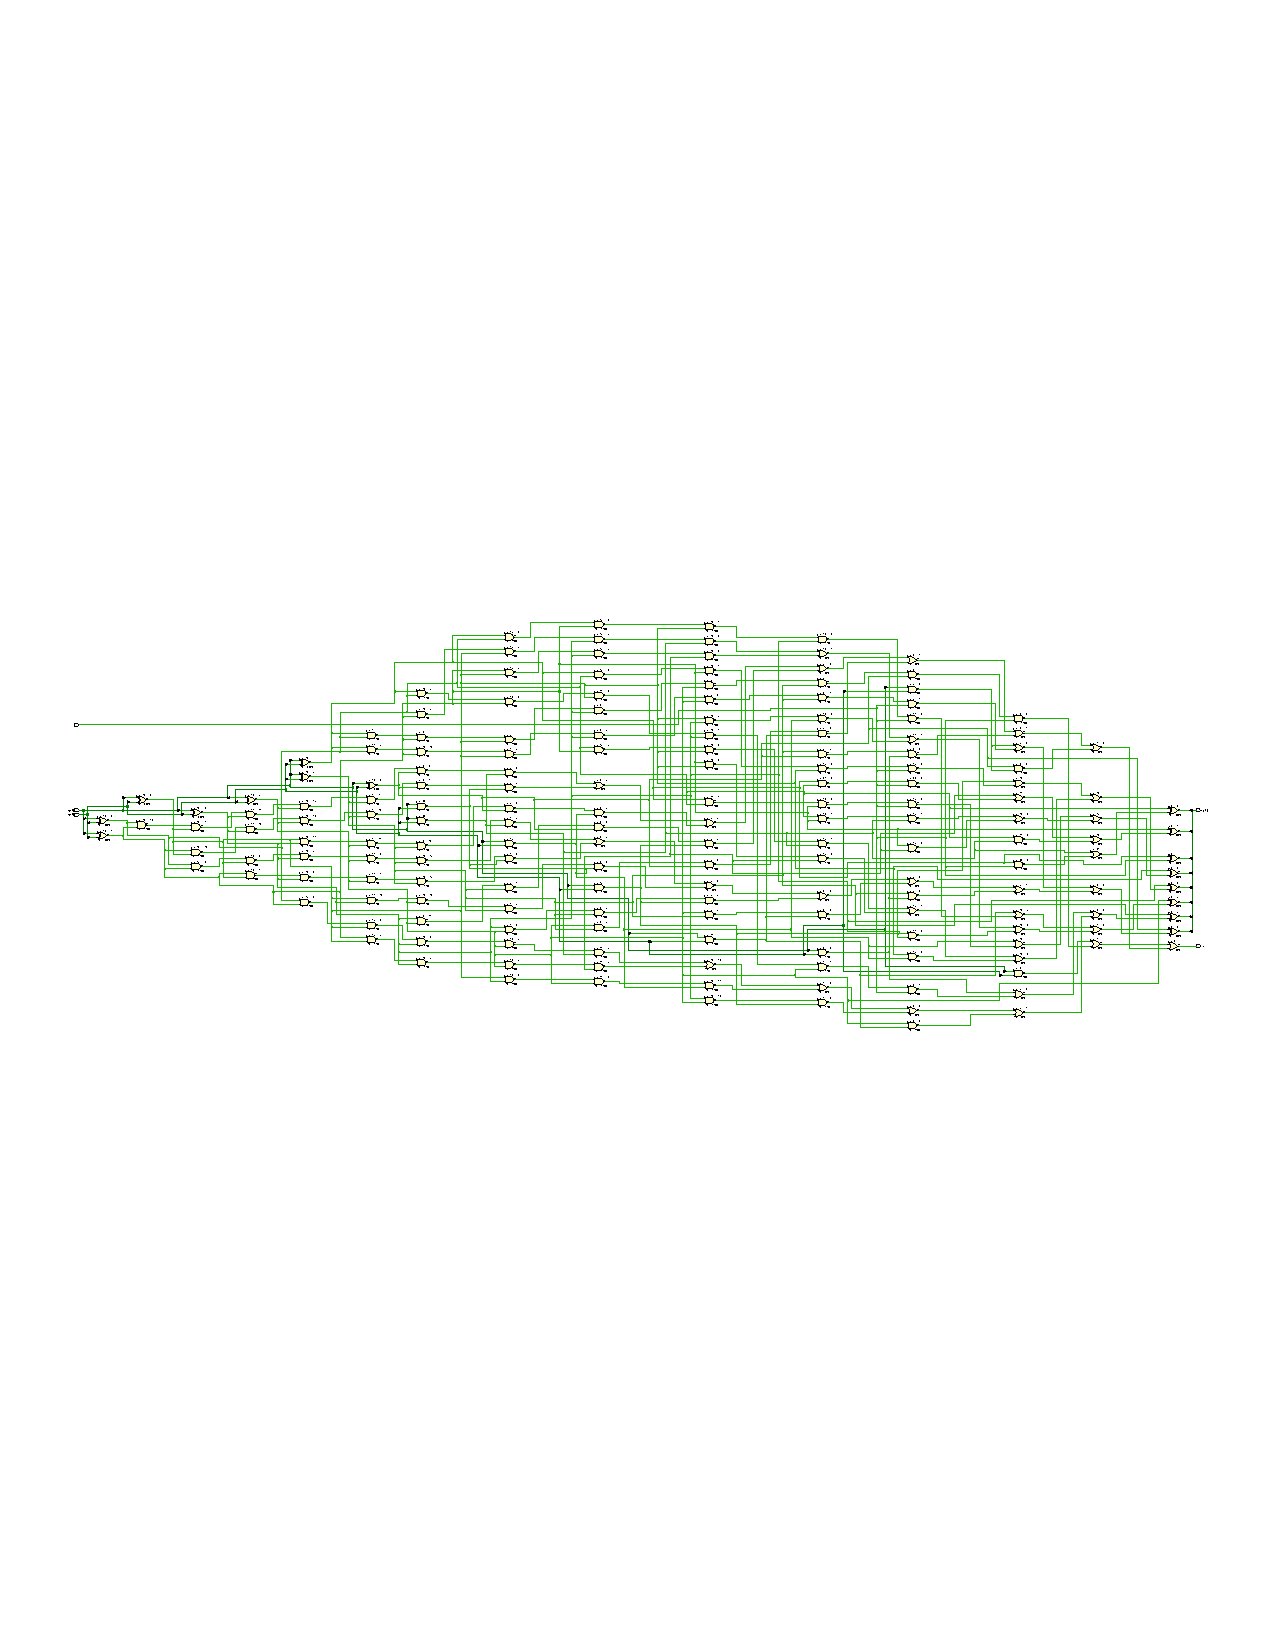
\includegraphics[scale=0.7]{sources/rtlDiagram.pdf}
    \textit{Diagrama RTL del archivo VHDL del sumador con acarreo anticipado de 8 bits}
\end{center}
\section{Diagrama de Síntesis}
\begin{center}
    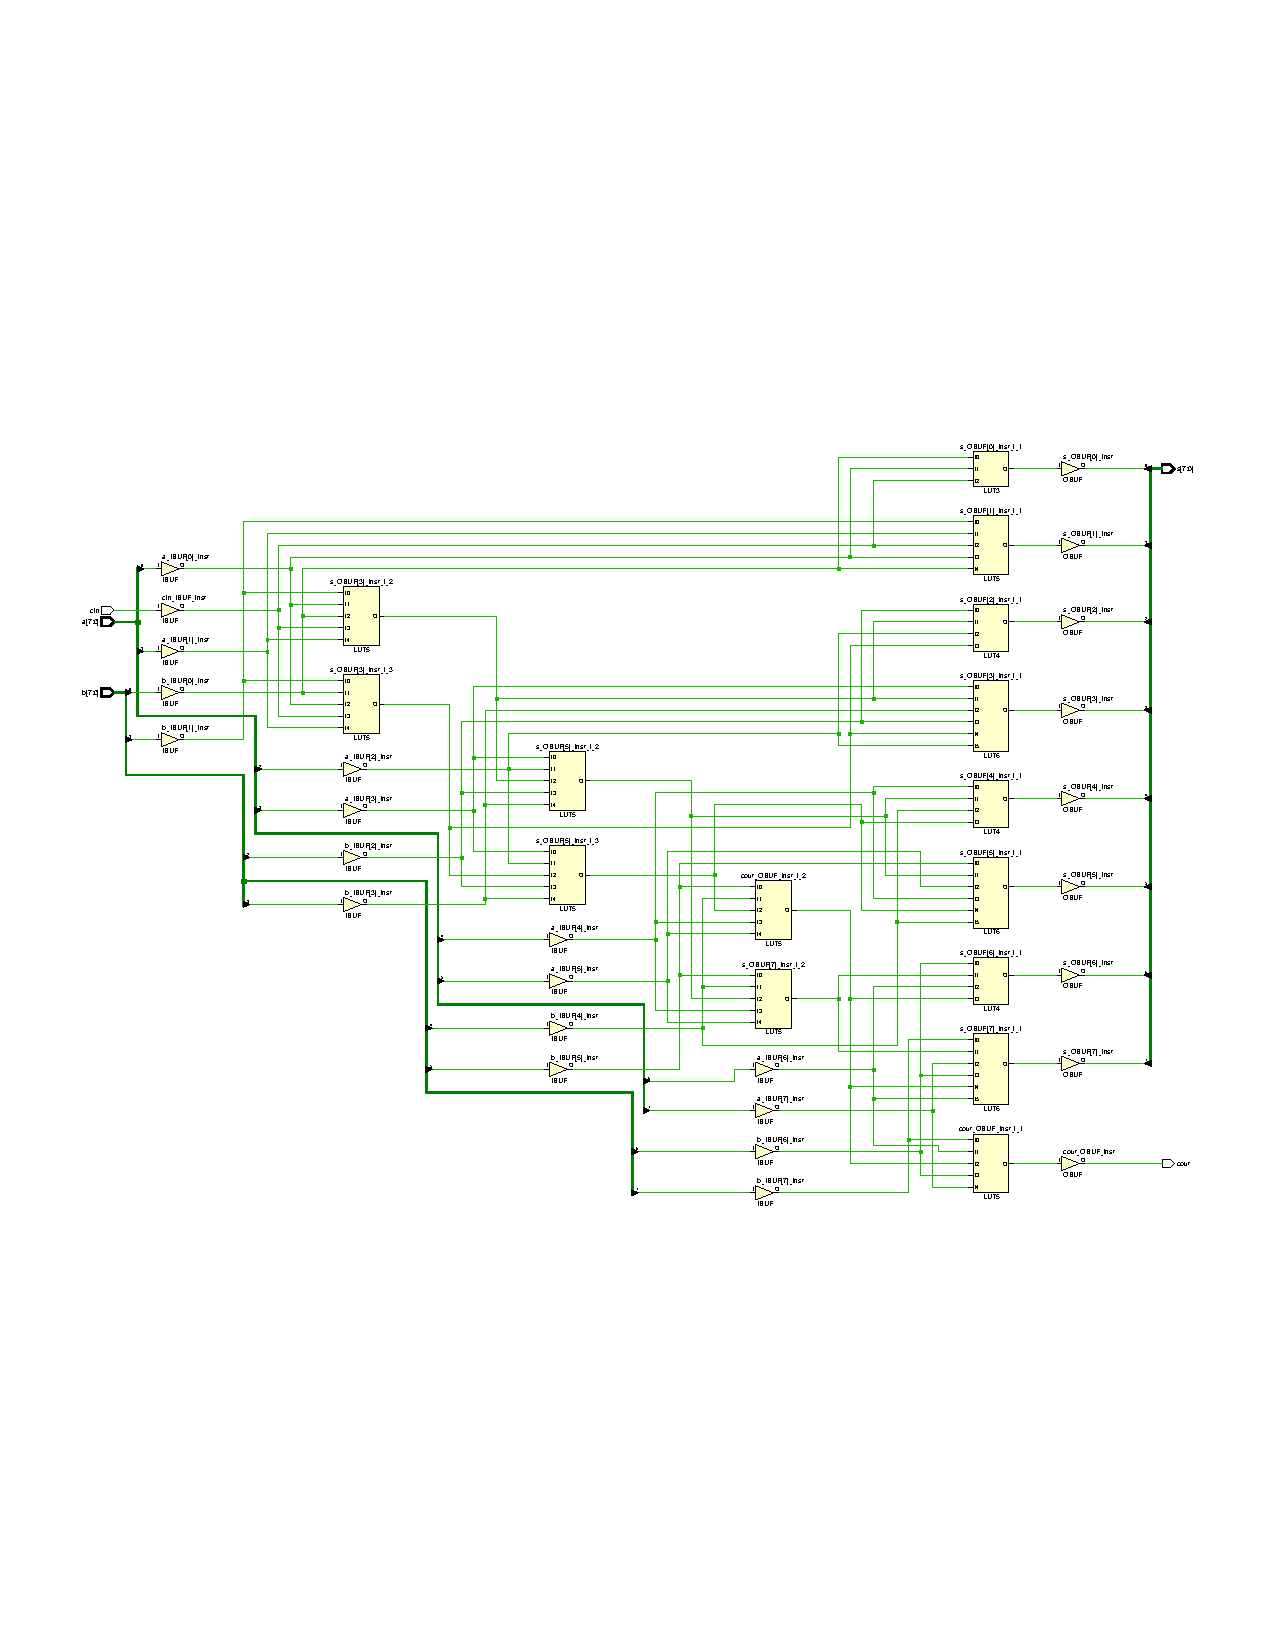
\includegraphics[scale=0.7]{sources/synthesisDiagram.pdf}
    \textit{Diagrama de Síntesis del archivo VHDL del sumador con acarreo anticipado de 8 bits}
\end{center}
\end{document}